\documentclass[11pt]{article}
\usepackage[margin=1in]{geometry}
\usepackage{amsmath,amssymb}
\usepackage{graphicx}
\usepackage{booktabs}
\usepackage{tabularx}
\usepackage{longtable}
\usepackage{caption}
\usepackage[table]{xcolor}
\usepackage{hyperref}
\hypersetup{colorlinks=true,linkcolor=black,urlcolor=blue!50!black}

\newcommand{\rch}{\langle r^2\rangle_{\rm ch}}
\newcommand{\Nc}{N_c}
\newcommand{\code}[1]{\texttt{\small #1}}
\newcommand{\statusline}{\textbf{Not yet in this table:} \code{fo\_baryon\_nlo}.  The run is in flight; the reference is already in the cross-checks.}


\title{GFMC charge form factors and radii:\\
       the $\alpha_s(m_Q)=0.1$ reference point and the $N_c$ scan}
\author{}
\date{\today}

\begin{document}
\maketitle

\section{What is measured, and in what convention}

The current is the number operator $J_N=\sum_k e^{i\mathbf q\cdot\mathbf x_k}$, and the
quantity quoted throughout is the \emph{one-body charge radius about the centre of mass},
\begin{equation}
  \rch \;=\; \frac1N\sum_k \big\langle (\mathbf r_k-\mathbf X)^2\big\rangle ,
  \qquad
  \frac{F(Q)}{F(0)} \;=\; \frac1N\sum_k \big\langle e^{i\mathbf q\cdot(\mathbf r_k-\mathbf X)}
  \big\rangle ,
\end{equation}
the same convention as \code{svm\_baryon.py}'s \code{<r\^{}2>\_ch} and \code{run/fit.py}.  For
a two-body state each constituent sits at $\pm\mathbf r/2$ from the centre of mass, so
$\rch=\langle r^2\rangle_{\rm rel}/4$.

Matrix elements come from a \emph{consistent-Gram} GEVP.  On the stored grid $t_k=k\Delta$ the
generator measures, on the same walkers,
\begin{equation}
  G_{ij}=\langle b_i|b_j\rangle = C_2(t_i+t_j),\qquad
  T_{ij}=\langle b_i|e^{-H\Delta}|b_j\rangle,\qquad
  M_{ij}=\langle b_i|J|b_j\rangle = C_J(t_i,t_j),
\end{equation}
with $|b_k\rangle=e^{-Ht_k}|\psi_T\rangle$; the ground-state Ritz vector solves
$Tv=\lambda Gv$ at the largest $\lambda$, and $J_{00}=v^\dagger Mv/v^\dagger Gv$.  Because $G$
and $M$ are one measurement, $F(0)=N$ holds \emph{identically} at every rank $m$ --- it is a
construction identity, not a test, which is why the rank is chosen from the $\rch$ plateau
instead.

Every pull quoted below is \textbf{fit-to-fit}: the identical fit is applied to the exact
reference $F(Q)/F(0)$ on the \emph{same} $Q$ grid, and the GFMC number is judged against that
target rather than against the true radius, so the ansatz bias is already contained in the
comparison.  The ``bias'' column records how large that effect is.

\section{Input parameters}

{\small
\begin{longtable}{@{}p{3.0cm}p{3.0cm}>{\raggedright\arraybackslash}p{9.6cm}@{}}
\toprule
parameter & value used & meaning \\
\midrule
\endfirsthead
\toprule
parameter & value used & meaning \\
\midrule
\endhead
\multicolumn{3}{l}{\emph{Physics inputs --- these define the theory}}\\
\code{--nf}        & $0$ & active flavours; the dark sector is quenched \\
\code{--Nc}        & $3$ (scan: $2\dots6$) & colours.  $C_F=(N_c^2-1)/2N_c$ \\
\code{--N\_coord}  & $2$ meson, $N_c$ baryon & constituents.  A colour-singlet baryon needs
  $N_{\rm coord}=N_c$ \\
\code{--alpha\_s}\newline \code{--alpha} & $0.1$ (MRS/FO)\newline $1$ ($N_c$ scan) & coupling at the scale
  $m_Q$ \\
\code{--OLO}       & LO / NLO & order of the MRS potential \\
\code{--mQ}        & $1$ & heavy-quark mass; a unit choice, since $\alpha_s(m_Q)$ fixes only
  $m_Q/\Lambda$ \\
\code{--mu}        & $0.0362001$ & $\mu_{\rm cut}$ in $\mu'(r)=\sqrt{\mu^2+\lambda^2/r^2}$,
  $=3.4\,\Lambda^{(2\text{-loop})}_d$.  \textbf{The default $2.0$ is a different theory}
  ($\rch=133.04$ instead of $56.69$) \\
\code{--mufac}     & $1$ & $\lambda$ in $\mu'(r)$ \\
\code{--masses}    & $[1,-1]$ meson, $[1]^{N}$ baryon & sign selects the pair colour channel:
  like signs $\to$ \code{'OA'} ($-\alpha C_F/(N_c{-}1)$ per pair), opposite $\to$
  \code{'OSing'} ($-\alpha C_F$) \\
\code{--potential} & \code{full} & \\
\code{--L}         & $0$ & infinite volume; the FV image sum is unreachable \\
\midrule
\multicolumn{3}{l}{\emph{Trial state and algorithm}}\\
\code{--Rstar}     & $0.35$ & scale at which the trial Bohr radius is set; degenerate with
  \code{spoila} \\
\code{--spoila}    & per config & trial width, $a_0=\texttt{spoila}\cdot2/V_B(R_*)$.  Tuned by
  radius matching, which the VMC scan showed \emph{is} the variational optimum \\
\code{--wavefunction} & \code{compact} & \\
\code{--dtau\_iMev}\newline \code{--n\_step}\newline \code{--count\_skip} & per config & step, steps, and
  the stride at which the two-time objects are stored ($N_\tau=$\,\code{n\_step}/\code{count\_skip}
  caps the usable rank) \\
\code{--n\_walkers} & $5000$ & \\
\code{--n\_skip}   & $50$ & Metropolis decorrelation \\
\code{--seed}      & $0$ (replicas $1,2$) & \\
\code{--no\_color\_vectors} & on & the singlet is an exact eigenvector of the colour structure,
  so this is bit-identical and far cheaper.  \textbf{Required} for $N_{\rm coord}>3$ \\
resampling         & off & branching desynchronises the two legs and corrupts $Q\neq0$ \\
\midrule
\multicolumn{3}{l}{\emph{Measurement and extraction}}\\
\code{--Q\_mag}, \code{--Q\_dir} & per config & current momentum \\
\code{--gevp\_cut} & $10^{-2}$ & Gram eigenvalue cut.  The \emph{measured} Gram is not positive
  definite, so $10^{-10}$ makes the GEVP explode; insensitive over $10^{-2}\dots10^{-1}$ \\
\code{--spike\_leverage} & $100$ & drop walkers with
  $\max_{ij}|w_{ij}|/\mathrm{median}\,|w_{ij}|$ above this \\
$m$ & plateau end & Krylov rank \\
\midrule
\code{--log\_mu\_r} & $1$ (FO NLO) & \textbf{not inert in the fixed-order generator}: it sets
  $V_B^{\rm NLO}=V_B[1+\tfrac{\alpha}{4\pi}(a_1+2\beta_0\log_{\mu r})]$ and hence the trial
  width $a_0$.  It \emph{is} dead in the MRS generator \\
\midrule
\multicolumn{3}{l}{\emph{Inert --- parsed but never referenced}}\\
\code{--spoilS},\newline \code{--Lcut}, \code{--g} & --- & \code{--spoilS} scales only the
  symmetric/octet channels, which the singlet build never selects \\
\bottomrule
\caption{Inputs.  Derived quantities the generator prints --- $\Lambda_d$, $\alpha_s(R_*)$,
$V_B(R_*)$, $a_0$ --- follow from these.}
\label{tab:inputs}
\end{longtable}}

\section{Results at $N_c=3$, $\alpha_s(m_Q)=0.1$}

\begin{center}\small
\begin{tabular}{llcr@{\,}c@{\,}lrrrr}
\hline\hline
potential & state & $m$ & \multicolumn{3}{c}{GFMC $\langle r^2\rangle_{\rm ch}$} & target & bias & reference & pull \\
\hline
FO & meson LO & 12 & 164.1 & $\pm$ & 2.96 & 168.8 & -0.00\% & 168.75 & -1.6$\sigma$ \\
FO & meson NLO & 12 & 84.97 & $\pm$ & 2.17 & 85.19 & +1.09\% & 84.269 & -0.1$\sigma$ \\
FO & baryon LO & 16 & 389.2 & $\pm$ & 6.35 & 382.1 & -0.15\% & 382.61 & +1.1$\sigma$ \\
MRS & meson LO & 16 & 56.88 & $\pm$ & 1.02 & 59.11 & +4.27\% & 56.6921 & -2.2$\sigma$ \\
MRS & meson NLO & 16 & 53.63 & $\pm$ & 0.981 & 54.6 & +4.86\% & 52.0713 & -1.0$\sigma$ \\
MRS & baryon LO & 16 & 114.6 & $\pm$ & 1.75 & 114.2 & -0.06\% & 114.252 & +0.3$\sigma$ \\
MRS & baryon NLO & 16 & 105.3 & $\pm$ & 1.54 & 103.1 & -0.05\% & 103.143 & +1.4$\sigma$ \\
\hline\hline
\end{tabular}

\end{center}
\captionof{table}{Charge radii at the reference mass.  ``target'' is the like-for-like value: the same
fit applied to the exact $F(Q)/F(0)$ on the same $Q$ grid; ``bias'' is how far that target sits
from the true reference, i.e.\ the fit-form systematic.  The $p=2$ dipole is exact for the
Coulomb meson (bias $0.00\%$) but \emph{not} for MRS, where it inflates the radius by
$4\!-\!5\%$ over $Q\le0.4$; the free-$p$ dipole is faithful for baryons ($\le0.4\%$).  A
$z$-expansion with $k_{\max}=4$ removes the ansatz dependence entirely and is quoted in the
cross-checks.  \statusline}
\bigskip

\noindent\textbf{The one live tension.}  Both NLO rows sit high by $\sim2\%$ while both LO rows
are at zero, and an independent run reproduces it.  It is not the fit ansatz: the free-$p$
dipole is unbiased on the exact $F$ to $0.05\%$, and a $k_{\max}=4$ $z$-expansion moves the
baryon NLO pull from $+1.5\sigma$ to $+1.6\sigma$.  Nor is it a convention mismatch in the
potential --- the Numerov and variational references \emph{exec the generator} and take
$V_B^{\rm NLO}$ out of its namespace, so the reference uses a bit-identical potential.  The
sharpest, ansatz-free statement is $(1-F)/(1-F_{\rm exact})$ at the lowest $Q$, which tends to
the radius ratio as $Q\to0$:
\begin{center}\small
\begin{tabular}{llll}
\toprule
 & LO & NLO \\
\midrule
MRS meson  & $0.987\pm0.019$ & $1.013\pm0.021$ \\
MRS baryon & $1.006\pm0.015$ & $1.021\pm0.015$ \\
\bottomrule
\end{tabular}
\end{center}
Never more than $1.4\sigma$, and $1.2\sigma$ after the $1.15\times$ error inflation measured
from a 16-seed replica study.  It is a $\sim1\sigma$ effect that happens to appear twice with
the same sign.

\section{Cross-checks}

\begin{center}\scriptsize
\begin{tabularx}{\textwidth}{>{\raggedright\arraybackslash}Xlll}
\hline\hline
check & measured & expected & verdict \\
\hline
$F(0)=N$ identity (consistent-Gram GEVP) & $\max|F(0)-N| = 4\times10^{-16}$ & $0$ exactly & machine precision \\
$F(0)=N$ at $N_{\rm coord}=N_c=5$ & $5.0000000000$ & $5$ & exact \\
\hline
\texttt{svm\_nbody.py} $N=2$ vs closed form & $-0.44443853$, $1.6875501$ & $-4/9$, $27/16$ & $6\times10^{-6}$ \\
\texttt{svm\_nbody.py} $N=3$ vs published Coulomb baryon & $3.8260983$ & $3.826$ & all digits \\
\texttt{svm\_nbody.py --potential fo\_nlo} $N=2$ vs \texttt{fo\_two\_body.py} & $-0.010609125$, $84.269834$ & $-0.010609161$, $84.269031$ & $1\times10^{-5}$ \\
\texttt{mrs\_two\_body.py} vs \texttt{svm\_baryon.py} $N=2$ (MRS LO) & $56.69186$ & $56.692063$ & $4\times10^{-6}$ \\
\hline
$N_c=3$ baryon: $\alpha=1$ vs $\alpha=0.1$ rescaled & $3.897\pm0.063$ & $3.892\pm0.059$ & $0.06\sigma$ \\
$N=2$: baryon path ($\kappa=3/4$) vs meson path rescaled & $5.210\pm0.096$ & $5.186\pm0.098$ & $0.2\sigma$ \\
\hline
FO meson LO vs closed form $27/(16\alpha^2)$ & $164.1\pm2.96$ & $168.8$ & $-1.6\sigma$ \\
FO meson NLO vs \texttt{fo\_two\_body.py} & $84.97\pm2.17$ & $85.19$ & $-0.1\sigma$ \\
FO baryon LO vs \texttt{svm\_nbody.py} & $389.2\pm6.35$ & $382.1$ & $+1.1\sigma$ \\
MRS meson LO vs Numerov / SVM $N\!=\!2$ & $56.88\pm1.02$ & $59.11$ & $-2.2\sigma$ \\
MRS meson NLO vs Numerov / SVM $N\!=\!2$ & $53.63\pm0.981$ & $54.6$ & $-1.0\sigma$ \\
MRS baryon LO vs SVM $N\!=\!3$ & $114.6\pm1.75$ & $114.2$ & $+0.3\sigma$ \\
MRS baryon NLO vs SVM $N\!=\!3$ & $105.3\pm1.54$ & $103.1$ & $+1.4\sigma$ \\
\hline
$\alpha=1$ baryon $N_c=2$ vs exact & $5.21\pm0.0961$ & $5.333$ & $-1.3\sigma$ \\
$\alpha=1$ baryon $N_c=3$ vs SVM & $3.895\pm0.0643$ & $3.82$ & $+1.2\sigma$ \\
$\alpha=1$ baryon $N_c=4$ vs SVM & $2.693\pm0.0309$ & $2.709$ & $-0.5\sigma$ \\
$\alpha=1$ baryon $N_c=5$ vs SVM, unconverged & $2.005\pm0.0219$ & $2.007$ & $-0.1\sigma$ \\
\hline
dipole fit-form bias on the exact $F$ (baryons) & $\le 0.40\%$ & $0$ & controlled via \texttt{--ref\_ff} \\
$z$-expansion ($k_{\max}=4$) fit-form bias & $\le 0.06\%$ & $0$ & ansatz-independent \\
walker state-ID: $\Delta J$ dropping the loudest walker & $\le 0.10\sigma$ & $\ll 1\sigma$ & ensemble average \\
walker state-ID: $N_{\rm eff}/N$, negative Ritz weights & $\ge 0.87$, 0\% & $1$, $0\%$ & healthy \\
$1/(\kappa\sqrt{\langle r^2\rangle})$ linear in $N_c$ & $+0.1763+0.1994N_c$ & exact linearity & $\sim2\%$ curvature \\
\hline\hline
\end{tabularx}

\end{center}
\captionof{table}{Validation.  The $\alpha$-rescaling entry is the sharpest: pure Coulomb scales exactly
($E\propto\alpha^2$, $\rch\propto\alpha^{-2}$, $F$ a function of $q/\alpha$), so the $N_c=3$
baryon run at $\alpha=1$ and the independent $\alpha=0.1$ campaign must agree after rescaling
--- they do, to $0.06\sigma$, across $10\times$ in $\alpha$, $100\times$ in $d\tau$ and
different seeds.}
\bigskip

\section{The $N_c$ scan, in $\alpha=1$ Coulomb units}

Because Coulomb scaling is exact, one set of runs at $\alpha=1$ covers every coupling.  Inside
the totally antisymmetric $N_{\rm coord}=N_c$ singlet each pair sits at $V(r)=-\kappa_N/r$ with
\begin{equation}
  \kappa_N=\frac{\alpha C_F}{N_c-1}=\frac{N_c+1}{2N_c}\Big|_{\alpha=1} .
\end{equation}
\emph{$\kappa_N$ is dimensionless}: with $\hbar=c=1$ the $1/r$ already carries the energy, and
in the code the potential is literally \code{-VB/norm\_R} with \code{VB} a pure number (in the
MRS generator $m_\psi$ enters only inside $V_B(r m_\psi)$, which is itself dimensionless).  The
quark mass appears in what \emph{follows} from $\kappa$, not in $\kappa$:
\begin{equation}
  a_0=\frac{1}{\mu\kappa_N}=\frac{2}{m_\psi\kappa_N},\qquad
  E_0 \sim -\frac{m_\psi\kappa_N^2}{4},\qquad
  \rch \sim \frac{1}{(m_\psi\kappa_N)^2},
\end{equation}
with $\mu=m_\psi/2$ the pair reduced mass.  So the dimensionless combinations are
$m_\psi^2\rch$, $E_0/m_\psi$, and $Q/(m_\psi\kappa_N)$ --- and since $\kappa_N\propto\alpha$,
$Q^2/(m_\psi^2\alpha^2)$ is $\alpha$-independent at fixed $N_c$, which is the abscissa of
Fig.~1 (left).  All numbers in this document are quoted at $m_\psi=1$.

At $N_c=2$, $\kappa_N=3\alpha/4$ --- and the $q\bar q$ singlet coupling $\alpha C_F$ is
\emph{also} $3\alpha/4$ there, so the diquark and the meson are the same Coulomb problem and
the $N=2$ end of the sequence is closed form,
\begin{equation}
  a_0=\frac{2}{m_\psi\kappa}=\frac{8}{3m_\psi\alpha},\qquad
  \rch=\frac34 a_0^2=\frac{3}{(m_\psi\kappa)^2}=\frac{16}{3m_\psi^2\alpha^2},
\end{equation}
which is $16/3$ at $\alpha=1$.  Since $\kappa_N\propto\alpha$, the $\alpha$-independent
combinations are $\alpha^2m_\psi^2\rch$ --- the ordinate of Fig.~2 (left), and the convention
in which the reference tables quote radii --- and $1/(m_\psi\kappa_N\sqrt{\rch})$, the
ordinate of Fig.~2 (right).

\begin{center}
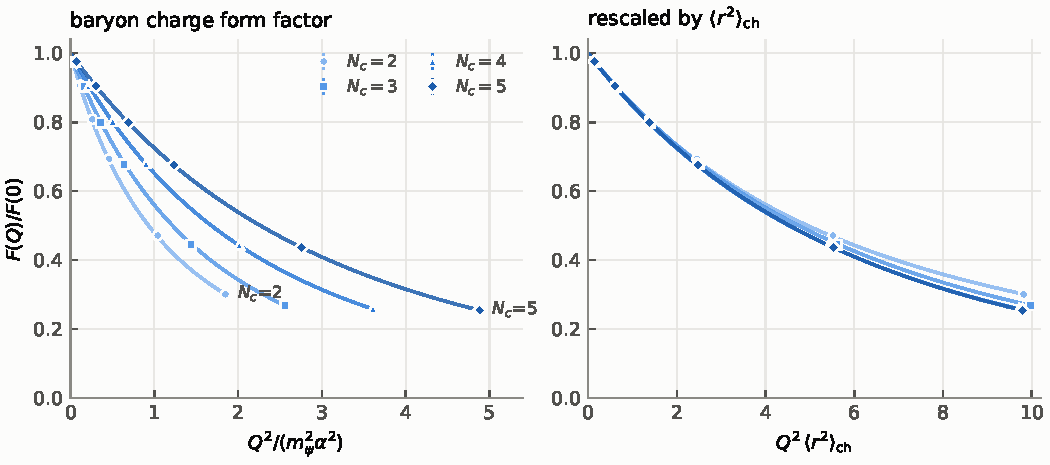
\includegraphics[width=\textwidth]{fig_baryon_ff.pdf}
\end{center}
\captionof{figure}{Baryon charge form factors.  Points are GFMC (5000 walkers, errors from a block
bootstrap that refits every resample); curves are the exact ($N_c=2$) or variational
($N_c=3,4,5$) references, anchored at $F(0)/F(0)=1$.  Colour is a one-hue ordinal ramp because
$N_c$ is ordered, and marker shape repeats the identity so nothing is colour-alone.  Reference curves are
evaluated on a dense grid, not interpolated between the six measured points.  Left: the
abscissa $Q^2/(m_\psi^2\alpha^2)$ is $\alpha$-independent, so the panel holds at any coupling
and what it shows is the genuine $N_c$ dependence, which enters through $C_F/(N_c-1)$.  Right:
the same data against the dimensionless $Q^2\rch$ --- the shape is nearly $N_c$-independent
once the scale is divided out, which is why the $Q$ grids were chosen matched in this
variable.}
\bigskip

\begin{center}
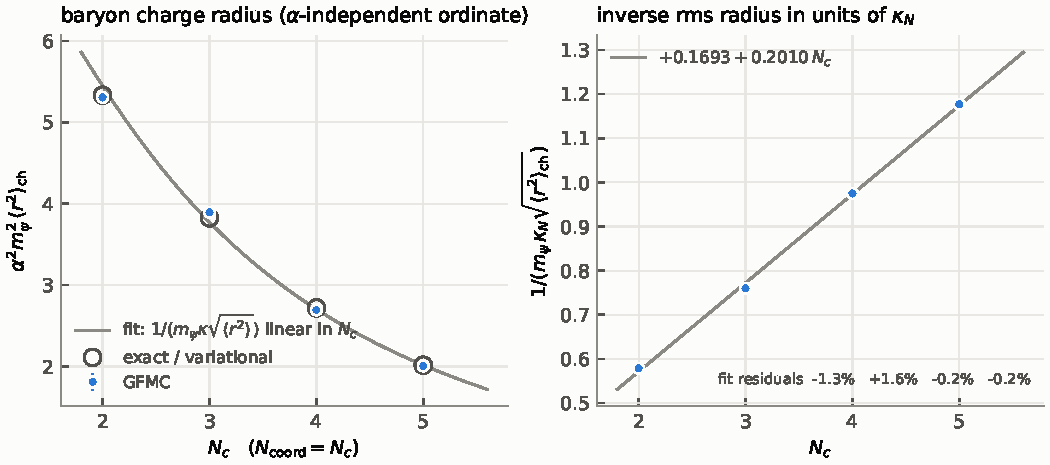
\includegraphics[width=\textwidth]{fig_radius_vs_nc.pdf}
\end{center}
\captionof{figure}{Left: the charge radius against $N_c$, with the reference values (open) and the fitted
law (grey).  Right: where the claim actually lives --- the dimensionless inverse rms radius
$1/(m_\psi\kappa_N\sqrt{\rch})$ is linear in $N_c$, i.e.\ \textbf{the baryon shrinks like $1/N_c$}.  The
residuals show the linearity is good to $\sim2\%$ but not exact.  A blind test makes the same
point: fitted on $N_c=2,3,4$ alone the law predicts $\rch(N_c{=}5)=2.053$, against a measured
$2.006\pm0.022$ --- $-2.3\%$, $-2.1\sigma$.  Extrapolations beyond the measured range should
therefore not be quoted more tightly than a couple of percent.}
\bigskip

\paragraph{Status.}  $N_c=6$ is running ($n_{\rm step}=430$, $d\tau=0.003719$,
\code{spoila}$=1.018416$, $Q=0.31\dots2.51$); its inputs are extrapolated from the two scaling
laws above rather than measured, so it is a genuine prediction test.  $N_c\ge5$ has no
converged variational reference by choice --- the method is anchored at $N_c=3$, where it
reproduces $3.826$ and passes the $\alpha$-rescaling null test, and carried forward with the
$m$ plateau and the walker state-ID diagnostics at every $N_c$.  Two seed replicas at $N_c=2$
are in flight to test whether the $-2.3\%$ there is a seed fluctuation or a systematic of the
exact-trial case, where the trial \emph{is} the eigenstate, the Gram is numerically rank-one
and $m$ therefore has nothing to project.

\end{document}
